% 1962 年全国卷第 9 题：正方体对角线 A_1C 与垂足 E。
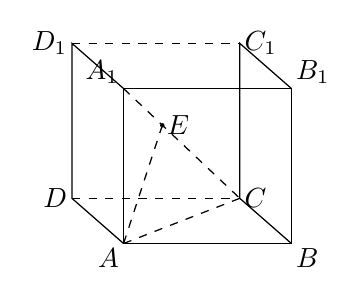
\begin{tikzpicture}[scale=0.82, line width=0.45pt,
  every node/.style={inner sep=1.5pt}]
  \coordinate (A) at (0,0);
  \coordinate (B) at (2.6,0);
  \coordinate (B1) at (2.6,2.4);
  \coordinate (A1) at (0,2.4);
  \coordinate (D) at (-0.8,0.7);
  \coordinate (C) at (1.8,0.7);
  \coordinate (C1) at (1.8,3.1);
  \coordinate (D1) at (-0.8,3.1);
  \coordinate (E) at (0.6,1.83);
  \draw (A)--(B)--(B1)--(A1)--cycle;
  \draw (A)--(D)--(D1)--(A1);
  \draw (B)--(C)--(C1)--(B1);
  \draw[dashed] (D)--(C) (D1)--(C1);
  \draw[dashed] (A1)--(C) (A)--(C) (A)--(E);
  \fill (E) circle (0.035);
  \node[anchor=north east] at (A) {$A$};
  \node[anchor=north west] at (B) {$B$};
  \node[anchor=west] at (C) {$C$};
  \node[anchor=east] at (D) {$D$};
  \node[anchor=south east] at (A1) {$A_1$};
  \node[anchor=south west] at (B1) {$B_1$};
  \node[anchor=west] at (C1) {$C_1$};
  \node[anchor=east] at (D1) {$D_1$};
  \node[anchor=west] at (E) {$E$};
\end{tikzpicture}
